\paragraph{Model merging is everywhere, but nobody knows the limit.}
Low-Rank Adaptation~\cite{hu2022lora} has made it routine to maintain
dozens of task-specific fine-tunes per base model, and \emph{merging}
those fine-tunes into a single deployable model has become the
dominant practical question. Task Arithmetic~\cite{ilharco2023task},
TIES~\cite{yadav2023ties}, DARE~\cite{yu2024dare},
KnOTS~\cite{stoica2025knots}, DO-Merging~\cite{domerging2025},
Core~Space~\cite{panariello2025core}, Task-Vector
Quantization~\cite{kim2025tvq}, and 1-bit-Merging~\cite{bit1merging2025}
all compete on this problem; each proposes an encoder, tunes
hyper-parameters, and reports benchmark numbers. Two operational
questions go unanswered. First, \emph{how much room is left}: a
method's benchmark score says nothing about whether a better merger
could still halve its error or whether it is already near optimal.
Second, \emph{when a method will fail}: a merger that wins on one base
can invert to worst-of-the-matrix on another with no warning. Both
reduce to a prior question no method addresses --- at a given storage
budget, what is the best \emph{possible} merging algorithm, and how far
from it are the methods we use today?

\paragraph{Contribution in one sentence.} \emph{Using a worst-task
rate-distortion analysis of LoRA merging as a lens, we build a merge
encoder (\textsc{rd-encoder ridge}) with the lowest worst-task NLL
excess of every method at its default hyperparameters on every base we
test, and a one-CPU-minute audit of any
trained adapter cohort that predicts when classical methods such as
TIES invert from best to worst --- with the threshold's upper edge and
ambiguous interior confirmed on three bases (one above the window
inverts, two inside stay ambiguous), one of them a pre-registered\footnote{Throughout,
\emph{pre-registered} means the prediction was committed to our
timestamped, version-controlled experiment log \emph{before} the
corresponding compute was run; the audit trail of
\S\ref{subsec:exp-T-scaling} shows no result commit predating the
registration.} out-of-sample third.}

\begin{figure}[t]
\centering
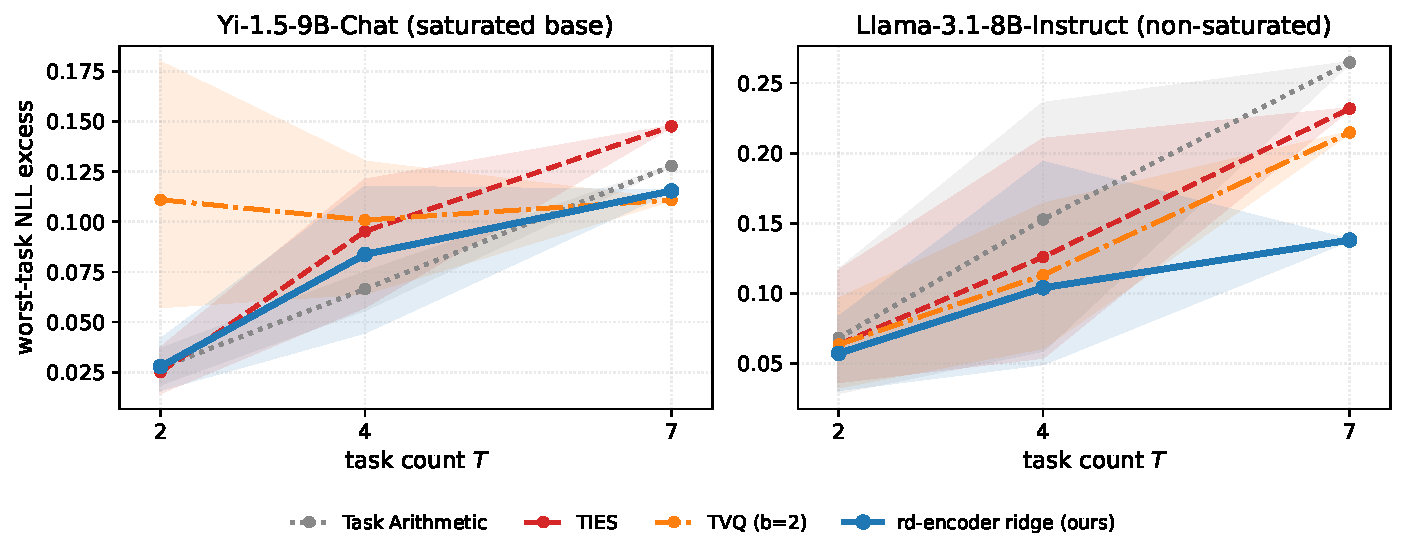
\includegraphics[width=0.92\textwidth]{../paper_artifacts/figures/figure1_cross_model_T_scaling.pdf}
\caption{\textbf{Same merge methods, opposite outcomes across bases.}
Worst-task NLL excess vs.\ task count $T \in \{2, 4, 7\}$ on three bases
ordered by per-task sign-election win-share range $R$: a saturated base
(left, Yi-1.5-9B-Chat, $R = 0.077$), the pre-registered third base
(middle, Mistral-7B-v0.3, $R = 0.0326$), and a non-saturated base
(right, Llama-3.1-8B-Instruct, $R = 0.028$); shaded by per-subset
min/max across the random task subsets per $T$. On Yi, TIES rises
sharply at $T = 7$ to become the \emph{worst} method, an inversion we
trace to per-task sign-election win-share concentration on saturated
bases (\S\ref{subsec:exp-T-scaling}; theoretical threshold derived in
Appendix~\ref{app:sign-election-threshold}). On Mistral, whose $R$ sits
inside the pre-registered ambiguity window $[0.025, 0.075]$, TIES is
neither best nor worst at $T = 7$, exactly as pre-registered. On Llama,
\textsc{rd-encoder ridge} (ours) widens its lead from a ratio of
$0.84$ at $T = 2$ to $0.52$ at $T = 7$ over Task Arithmetic, the
cleanest cross-$T$ signal in our matrix; the same salvage strengthens
on Mistral ($1.38 \to 0.82 \to 0.47$).}
\label{fig:hero}
\end{figure}

\paragraph{Two deliverables, one analysis.} We answer both questions
with a single rate-distortion analysis of merging, and the payoff is
operational before it is theoretical. \emph{A method.} The analysis
comes with an exact-construction encoder; on real adapters that exact
construction fails for a measured spectral reason, but a one-line
Tikhonov ridge salvages it into \textsc{rd-encoder ridge}, a merge
method that ties or beats every published baseline at $T = 4$ on the
$4$-base $\times$ $7$-method matrix we evaluate and \emph{widens} its
lead as the task count grows (excess ratio vs.\ Task Arithmetic
$0.84 \to 0.68 \to 0.52$ over $T \in \{2, 4, 7\}$ on
Llama-3.1-Instruct; Figure~\ref{fig:hero}). \emph{An audit.} The same
analysis yields a one-CPU-minute diagnostic that predicts \emph{when} a
classical method will fail: a perturbation derivation of the TIES
sign-election update gives a closed-form ambiguity window
$R^\star \in [0.025, 0.075]$ on a cohort's per-task win-share range,
and TIES inverts from best to worst exactly when a cohort rises above
it. The window predicts inversion above it and ambiguity inside it:
Yi-Chat ($R = 0.077$, above) inverts, while Llama-Instruct
($R = 0.028$) and a pre-registered Mistral-7B-v0.3 ($R = 0.0326$),
both inside, stay ambiguous --- TIES neither inverting nor winning.
The below-window regime (where the model predicts TIES wins outright)
is untested.
Compressed into a five-rule decision tree
(\S\ref{sec:practical-recommendations}), the audit tells a practitioner
which merger to use and which task sets not to merge at all. We now
describe the analysis these come from.

\paragraph{The lens: merging as compression.} Both deliverables come
from treating merging as a
compression problem: $T$ task-specific weight updates must be encoded
into a single model within a storage budget, and quality is the loss
inflation on the \emph{worst}-affected task (a merged model that
collapses on one task is not a useful deployment target). For this
problem we prove lower and upper bounds that match in their rate
exponent (up to a factor in $T$ in the constant, conjectured tight)
-- a rate-distortion theorem -- with a closed-form answer that
separates worst-task error
into two parts with different cures. The first is an
\textbf{irreducible floor} set entirely by the geometry of the tasks:
if the tasks' weight subspaces overlap, no encoder at any bit budget
can drive worst-task error below it; serving such tasks from one
merged model is information-theoretically impossible to do well, and
the right response is to not merge them. The second is a
\textbf{compression term} that decays exponentially in the bit budget
and that an explicit, practical encoder -- randomized orthogonal
mixing followed by uniform scalar quantization -- achieves up to a
constant factor. The dichotomy gives merging research a diagnostic it
has not had: measure the overlap, and you know whether a task set is
limited by \emph{information} (the floor; change the task set) or by
\emph{algorithms} (the gap above the floor; build a better merger).

\paragraph{Which regime is real merging in? We measure it.} We train
$16$ LoRA adapters -- four base models (Llama-3.1-8B, Qwen-2.5-7B,
Mistral-7B, Yi-1.5-9B) $\times$ four tasks -- and measure the overlap
quantity the theorem identifies. The answer is unambiguous: real task
subspaces are linearly \emph{independent} in every layer of every
model. The floor is exactly zero; practical merging lives entirely in
the algorithm-limited regime. This turns the theorem into a measured
verdict on current practice: the five standard methods we evaluate
leave $0.10$--$0.22$ nats/token of worst-task error on the table
(bootstrap $95\%$ CIs), and \emph{none of it is an
information-theoretic floor} -- the bound's floor is zero, so the gap
is distance from the optimum, not an unavoidable cost of merging. (How much of that slack a \emph{practical} encoder
reclaims is the achievability question of
\S\ref{subsec:exp-rd-encoder}, where the exact optimal construction
in fact fails on real adapters and a one-line regularized variant
reclaims a measurable fraction.) Zero overlap also predicts which
methods can work: subspace-alignment merging
(KnOTS~\cite{stoica2025knots}) has nothing to exploit and is
statistically indistinguishable from naive averaging, exactly as the
theory says, while TIES -- which attacks sign-level interference
instead -- is the only method that separates from the baseline. What
\S\ref{sec:exp} validates on real LLMs is thus the regime
\emph{diagnosis} and its qualitative consequences --- which methods
can work --- not the quantitative rate-distortion curve, whose
compression slope is operationally invisible at the bit budgets
merging uses (\S\ref{subsec:exp-lora}).

\emph{A worked example.} A Llama-3.1-8B base with $T{=}4$ rank-$16$
LoRAs has $\deff \leq Tr = 64$ relevant dimensions per layer. The
theory's two corners are: orthogonal task subspaces ($\deff = 64$,
floor $0$, quality limited by rate and algorithm) and fully shared
subspaces ($\deff = 16$, floor $\approx 0.75\,B^2$, a ceiling no
merger can break). Our measurements put all four models at
$\deff = 64$ in every layer -- the floor-zero corner -- so this
model's measured worst-task excess of $0.22$ nats/token is headroom,
not floor. The overlap-limited corner did not arise for any task set
we tried; identifying real task families that induce it is a
direction the theorem makes precise, and we return to it in
\S\ref{sec:discussion}.

\paragraph{The formal problem.} Fix $T$ tasks, ambient dimension $d$,
and LoRA rank $r \leq d$. Each task is a pair $(\tau_t, H_t)$: a task
vector $\tau_t \in \R^d$ (the LoRA update) and a positive-semidefinite
$H_t$ of rank $r$ (the task's Hessian or Fisher surrogate at
$\tau_t$), normalized so $\tau_t^\top H_t \tau_t \leq B^2$. An encoder
maps $(\tau_1, \ldots, \tau_T)$ to $R$ bits; a decoder reconstructs
one merged model $w^\star \in \R^d$; the per-task distortion
$D_t(w) := (w - \tau_t)^\top H_t (w - \tau_t)$ is the second-order
loss inflation from using $w$ in place of $\tau_t$. The
rate-distortion function $\mathcal{D}^\star(T, d, r, B, R)$ is the
infimum over encoder/decoder pairs of expected worst-task distortion
$\max_{t \leq T} D_t(w^\star)$, under a hard distribution on task
geometries in which the task subspaces are drawn uniformly at random
(Stiefel-random; \S\ref{sec:setup}). Two features separate this from
classical lossy source coding: the encoder observes $T$ sources, not
one (multi-description coding~\cite{elgamalcover1982md} treats
\emph{average} distortion, and Lemma~\ref{lem:id} shows max
dominates average, so the worst-task function is strictly larger);
and distortion is measured in task-specific rank-$r$ subspaces, so
the controlling quantity is the effective dimension
$\deff := \E[\rank(\sum_t P_{V_t})] \leq \min(Tr, d)$, attained
almost surely in the random-subspace model.

\paragraph{Contributions.}
\begin{enumerate}[leftmargin=*,topsep=2pt,itemsep=2pt]
\item \textbf{A merge method and a cohort audit, both falling out of
the bound (\S\ref{sec:exp}, \S\ref{sec:practical-recommendations}).}
\textsc{rd-encoder ridge} --- the achievability construction
regularized by one Tikhonov ridge term to survive a measured spectral
failure on real adapters --- matches or beats every published baseline
(within CI), including data-free RegMean, on every base we test. A
perturbation analysis of the TIES sign-election
yields a one-CPU-minute audit and a five-rule decision tree that
predict when classical mergers invert from best to worst, with the
upper threshold and ambiguous interior confirmed on three bases (one
inverting above the window, two ambiguous inside, one pre-registered).

\item \textbf{A reduction identity (Lemma~\ref{lem:id}).} For every
admissible $(\tau, H)$ and every $w$: worst-task distortion is at
least a quantization term around the $H$-weighted centroid plus a
spread term no encoder can remove. The identity is the bridge from
Shannon's single-source machinery to multi-source max-distortion:
the first term is what bits buy, the second is what no rate erases.

\item \textbf{The floor in closed form (Lemma~\ref{lem:floor-general}).}
Under the random-subspace hard distribution the irreducible spread
term equals $B^2(1 - \deff/(Tr))$ exactly: zero when subspaces are
independent ($\deff = Tr$), approaching $B^2(1 - 1/T)$ as they
coincide, and interpolating explicitly in between.

\item \textbf{A lower bound on every merging algorithm
(Theorem~\ref{thm:general}).} At rate $R$, no encoder/decoder pair
beats floor plus $c_{\mathrm{TQ}} \cdot (B^2 \deff / (Tr)) \cdot
2^{-2R/\deff}$, for arbitrary positive-definite per-task spectra. The
proof composes Yao's minimax principle, Lemma~\ref{lem:id}, a
reduction to $\range(\bar H)$, and an $O(d)$-equivariance argument.

\item \textbf{A rate-exponent-matching explicit algorithm
(Theorem~\ref{thm:achv}).}
In the floor-zero regime, randomized orthogonal mixing of the
$\bar H^{1/2}$-scaled centroid plus uniform scalar quantization
achieves the same $2^{-2R/(Tr)}$ decay, so
$\mathcal{D}^\star = \Theta(B^2 \, 2^{-2R/(Tr)})$ for fixed $T$; the
construction reduces to TurboQuant~\cite{zandieh2025turboquant} at
$T = 1$. The analysis gives the constant $C = Tc^2/3$; our
measurements (below) show the true $T$-dependence is logarithmic,
making the gap a sharply posed open problem rather than a loose end.

\item \textbf{Numerical validation of slopes and constants.} Monte
Carlo across $T \in \{2,3,4,8\}$, $d \in \{128, 512, 2048\}$,
$r \in \{4, 8, 16\}$ confirms the predicted exponent $-2R/\deff$ to
within $\pm 0.01$ (bootstrap $95\%$ CI, 1000 trials/cell). A dedicated
$T$-sweep ($T$ up to $16$, 1000 trials/cell) measures the
achievability constant's growth: \emph{logarithmic} in $T$
($R^2 \geq 0.998$ against $\log T$ in all cells; ratio at $T{=}16$
only $1.8\times$ that at $T{=}2$, against $8\times$ if linear), with
slope shrinking like $1/\sqrt{r}$ -- the signature of a max-of-$T$
concentration argument, which we state as a conjecture.

\item \textbf{A real-LLM calibration that turns the bound into a
measured gap (\S\ref{sec:exp}).} The $16$-adapter study above: floor
zero everywhere; $0.10$--$0.22$ nats/token of recoverable headroom;
only TIES separates from naive averaging, KnOTS does not (as
predicted at zero overlap); merging difficulty tracks the
pretraining/instruction-tuning recipe rather than attention design;
and a universal ``less-is-more'' regime in which $2$-bit task-vector
quantization beats higher-bit quantization on all four architectures.
\end{enumerate}

\paragraph{Scope and limitations.} The bound certifies a \emph{lower
envelope}, not a tight per-instance grade: real task vectors are more
benign than the worst case, so a method's gap to $\mathcal{D}^\star$
upper-estimates its suboptimality. The matching upper bound is proved
in the generic random-subspace regime with $Tr \leq d$; in the
floor-positive regime an explicit linear encoder achieves exponent
$2^{-2R/(\deff + |A| - 1)}$ and closing the gap to $2^{-2R/\deff}$
appears to require non-linear encoders
(Remark~\ref{rem:sharedv-gap}). The achievability constant's
$T$-dependence is now measured (logarithmic, contribution 6) but not
yet proved; tightening $Tc^2/3$ to match is open. The theory is
stated for quadratic loss; the bridge to cross-entropy via local
Fisher-quadratic approximation, and its measured residual, are
discussed in \S\ref{sec:discussion}.

\paragraph{Paper organization.} \S\ref{sec:setup} formalizes the
rate-distortion model and the hard distribution. \S\ref{sec:lower}
proves the lower bound. \S\ref{sec:achv} gives the matching
construction. \S\ref{sec:exp} reports synthetic validation and the
real-LLM calibration. \S\ref{sec:discussion} discusses the
cross-entropy bridge, the open exponent and constant gaps, and
implications for merging-algorithm design.
